\section*{Assignment 02: Network Effects and Launch Strategy}
\addcontentsline{toc}{section}{Assignment 02: Network Effects and Launch Strategy}

SkillSync runs on three loops. A cross-side effect keeps NGOs posting once students deliver; a student same-side effect grows through peer stories and cohort rituals \citep{Choudary2016}; and every project adds structured data that sharpens matching, pushing us toward the curated orchestrator pattern in \citet{Reillier2017}.

Seeding those loops meant tackling the penguin problem head-on. We signed two anchor NGOs for social proof \citep{HagiuWright2013}, recruited 40 founding students with concierge onboarding, and promised make-good support if a match fizzled. The package mirrors subsidy tactics from \citet{Gunasilan2024} and \citet{FarrellSaloner1986} so neither side felt like the first penguin off the ice.

The launch still taught humility. Casting the net too wide made the community feel thin, so a rerun would focus on one faculty, track time-to-first-value from day one \citep{ShapiroVarian1999}, and arm student ambassadors instead of impersonal emails. Figure~\ref{fig:application-flow} shows the streamlined application flow that underpins that learning: clear steps, no ``post and pray'' spam, and guidance chips that echo our mentoring tone.

\begin{figure}[h]
  \centering
  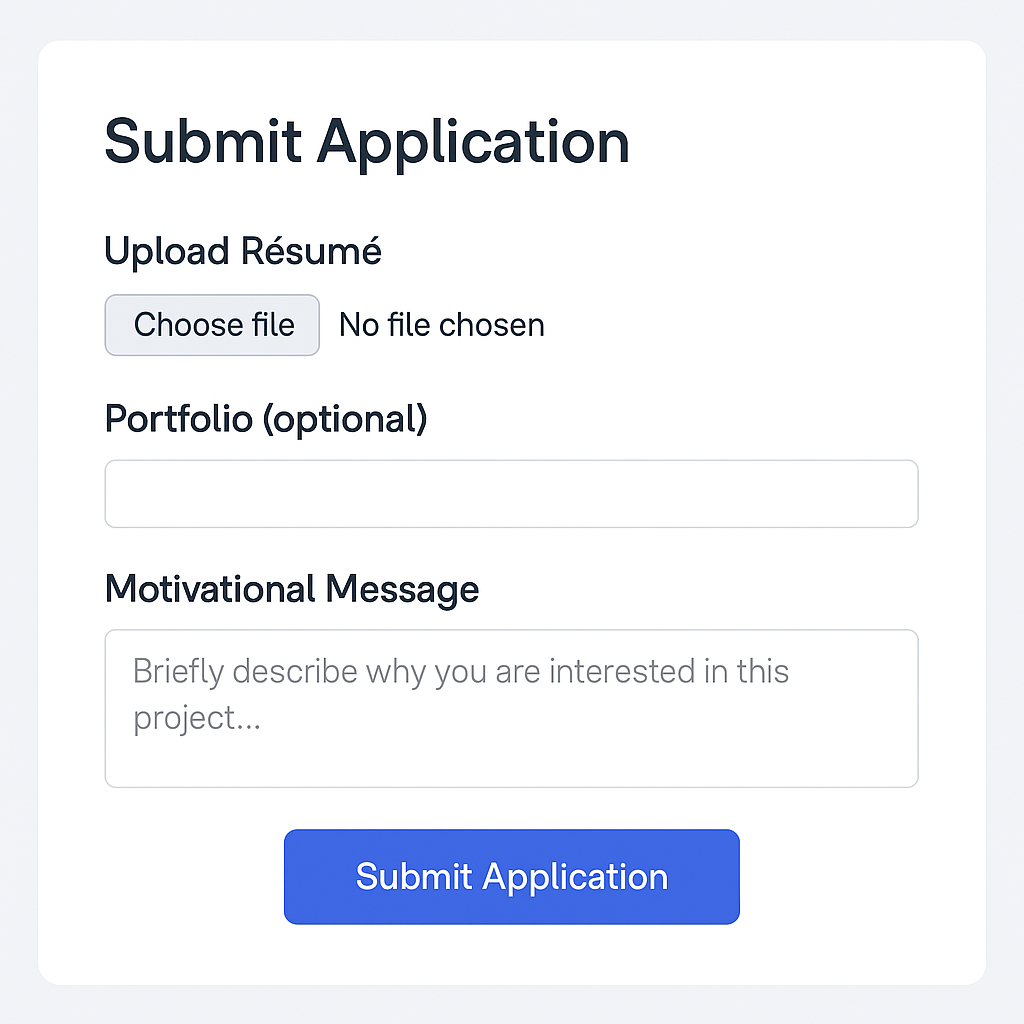
\includegraphics[width=0.85\linewidth]{figures/opgave02/ansoegningsflow.png}
  \caption{End-to-end student application flow (`ansoegningsflow.png`) used to trigger the first successful loops.}
  \label{fig:application-flow}
\end{figure}
